%!TEX root = ../Main.tex
% Project management
\chapter{Project Management} % (fold)
\label{apdx:project_mang}

\section{Interim Gantt Chart} % (fold)
\label{apdx:gantt_chart1}
	This Gantt chart (Figure~\ref{fig:gantt1}) was also presented in the interim report, and proved to be far too optimistic about the time certain tasks would take.
	\begin{sidewaysfigure}[tb]
		\begin{center}
			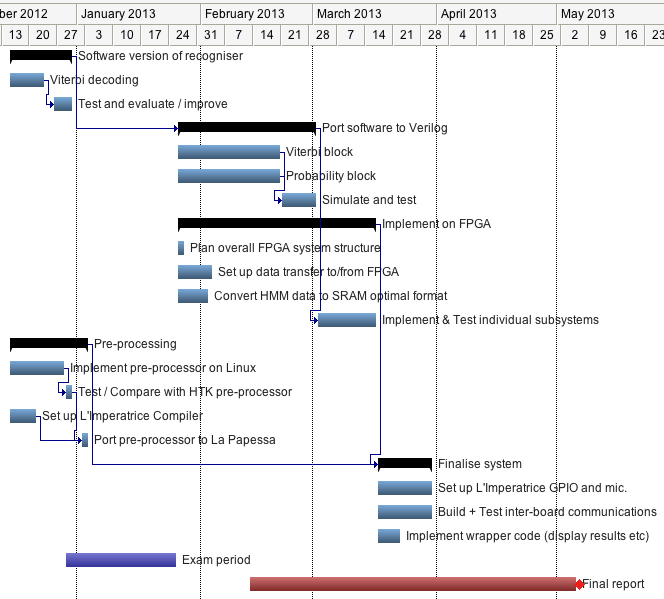
\includegraphics[height=0.6\textwidth]{gantt-chart-interim}
		\end{center}
		\caption{Interim Gantt chart}
		\label{fig:gantt1}
	\end{sidewaysfigure}

	\clearpage
% section gantt_chart1 (end)

\section{Final Gantt Chart} % (fold)
\label{apdx:gantt_chart2}
	This Gantt chart (Figure~\ref{fig:gantt2}) illustrates the rate of progress that was actually accomplished.
	\begin{sidewaysfigure}[tb]
		\begin{center}
			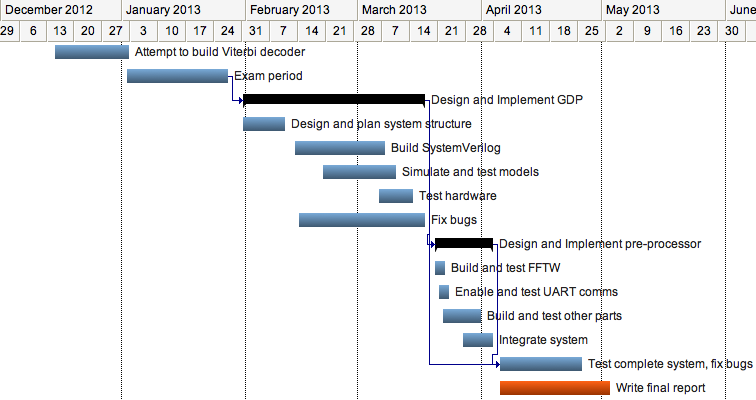
\includegraphics[height=0.4\textwidth]{gantt-chart-final}
		\end{center}
		\caption{Final Gantt chart}
		\label{fig:gantt2}
	\end{sidewaysfigure}

	\clearpage
% section gantt_chart2 (end)


\section{Git Commit Log} % (fold)
\label{apdx:git_commit_log}
Below is a log of the commits made to this project's git repository.

(2013-04-24) Restructured SystemVerilog into Synplify and Modelsim projects \\*
(2013-04-21) Added a program to test double to uint16\_t \\*
(2013-04-21) Wording tweaks, mainly additions to analysis. \\*
(2013-04-21) Fixed software normalisation (reversed subtraction) \\*
(2013-04-21) Added some appendix structure and content \\*
(2013-04-21) Started adding a fixed point version to GDP-in-C \\*
(2013-04-20) A bunch of writing, reorganisation, better appendices structure... \\*
(2013-04-20) Updated to use more senone data \\*
(2013-04-20) Added normalisation to feed\_obs, reformatted verilog senone data \\*
(2013-04-20) Fixed float->uint bug in D\_TO\_U16 \\*
(2013-04-20) Updated Main for the latest FPGA version \\*
(2013-04-20) Added a Copy target, to simplify things... \\*
(2013-04-19) Fixed bug in gconst extraction \\*
(2013-04-18) Added a software GDP and GPIO testing code \\*
(2013-04-18) Yay for writing \\*
(2013-04-17) More writing... \\*
(2013-04-16) Minor tweaks and patches to code, lots of report. Commit before refactoring Testing section. \\*
(2013-04-09) Mainly changes to System and Approach \\*
(2013-04-04) Added outlines to System, Testing, Appendices, and writing to Approach \\*
(2013-04-04) Fixed typo in Abstract \\*
(2013-04-03) More writing in Approach section. Mainly. \\*
(2013-04-03) Built a version of the GDP in C, tweaks to binary and extract lisps \\*
(2013-04-01) Removed mfc and wav files from git... \\*
(2013-03-31) Added missing chapter containers, Started trying to write... \\*
(2013-03-31) Added sampling from WAV files, tidied up system \\*
(2013-03-28) More introduction. Mainly. \\*
(2013-03-28) Tweaks to extract \\*
(2013-03-28) Integrated files, created Makefile \\*
(2013-03-25) Re-ran the voxforge adaptation, separated 48kHz wavs from the 8kHz wavs \\*
(2013-03-25) Added report structure and Tested FFTW \\*
(2013-03-18) Fixed mistake in new vector pin \#define \\*
(2013-03-18) Send and receive working correctly \\*
(2013-03-18) First attempt at the C application \\*
(2013-03-14) Hardware working. Normalise disabled \\*
(2013-03-13) Tweaks to plan after srg meeting \\*
(2013-03-12) Made Synplify versions of system, works in hardware, sometimes \\*
(2013-03-12) Added constraints list for La Papessa Rev C \\*
(2013-03-11) Made send state machine. Full send test with sram model - working. \\*
(2013-03-11) Added normaliser code, top level sram connections and sram testbench \\*
(2013-03-10) More SV, uart working now, started final report \\*
(2013-03-08) Changed uart to use num buffers, added Max module, etc \\*
(2013-03-08) Added top level SV code \\*
(2013-03-07) Added testbench and data generation, finished gdp controller + tester \\*
(2013-03-06) GDP works. Added more to binary utils \\*
(2013-03-04) Started SV conversion, added binary lisp code \\*
(2013-02-25) Added missing Verilog file \\*
(2013-02-25) Added Verilog, improvements to export.lisp \\*
(2013-02-12) More capabilities... or not \\*
(2013-01-31) Big messy commit. Most important: extract.lisp, citations \\*
(2012-12-12) Interim report, night before \\*
(2012-12-12) Updated Gaussian algo to use precomputed values \\*
(2012-12-11) Fixed error in bib \\*
(2012-12-11) Additions to report and more citations \\*
(2012-12-10) Added readme \\*
(2012-12-10) First huge commit \\*
% section git_commit_log (end)